\documentclass[tikz,border=4pt]{standalone}
\usepackage{amsmath,amssymb}
\usetikzlibrary{arrows.meta,calc,decorations.pathreplacing}
\definecolor{cA}{HTML}{924800}
\definecolor{cB}{HTML}{2F7FC8}
\definecolor{cC}{HTML}{39994B}
\tikzset{
  pt/.style={circle,fill=black,inner sep=0pt,minimum size=4pt},
  disp/.style={-{Stealth[length=2.6mm,width=2mm]},line width=0.9pt,shorten <=2.5pt,shorten >=2.5pt},
  lab/.style={font=\small,sloped,text=black},
  brc/.style={decorate,decoration={brace,amplitude=5pt,raise=3pt},line width=0.6pt},
}
\begin{document}
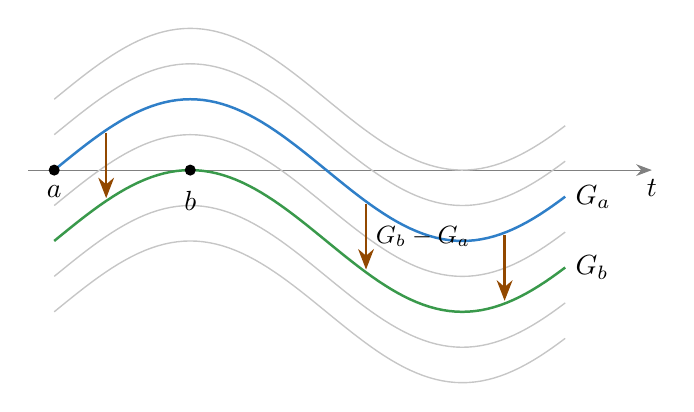
\begin{tikzpicture}[x=1.1cm,y=0.9cm]
  \draw[-{Stealth[length=2mm]},gray] (-0.3,0) -- (6.9,0) node[below,text=black]{$t$};
  \foreach \c in {-2,-1.5,-0.5,0.5,1} \draw[gray!45,line width=0.5pt,domain=0:5.9,samples=80] plot (\x,{sin(\x r)+\c});
  \draw[cB,line width=0.9pt,domain=0:5.9,samples=80] plot (\x,{sin(\x r)}) node[right,text=black]{$G_a$};
  \draw[cC,line width=0.9pt,domain=0:5.9,samples=80] plot (\x,{sin(\x r)-1}) node[right,text=black]{$G_b$};
  \foreach \t in {0.6,3.6,5.2} \draw[disp,cA,shorten <=1pt,shorten >=1pt] (\t,{sin(\t r)}) -- (\t,{sin(\t r)-1});
  \node[right,font=\small] at (3.6,{sin(3.6 r)-0.5}) {$G_b-G_a$};
  \node[pt,label=below:$a$] at (0,0) {};
  \node[pt,label={[label distance=2pt]below:$b$}] at ({pi/2},0) {};
\end{tikzpicture}
\end{document}
